\documentclass[nobib]{tufte-handout}

\title{Övningstillfälle 2: Programmeringsövningar $\cdot$ 1MA020}

\author[Vilhelm Agdur]{Vilhelm Agdur\thanks{\href{mailto:vilhelm.agdur@math.uu.se}{\nolinkurl{vilhelm.agdur@math.uu.se}}}}

\date{10 februari 2023}


%\geometry{showframe} % display margins for debugging page layout

\usepackage{graphicx} % allow embedded images
  \setkeys{Gin}{width=\linewidth,totalheight=\textheight,keepaspectratio}
  \graphicspath{{graphics/}} % set of paths to search for images
\usepackage{amsmath}  % extended mathematics
\usepackage{booktabs} % book-quality tables
\usepackage{units}    % non-stacked fractions and better unit spacing
\usepackage{multicol} % multiple column layout facilities
\usepackage{lipsum}   % filler text
\usepackage{fancyvrb} % extended verbatim environments
  \fvset{fontsize=\normalsize}% default font size for fancy-verbatim environments

\usepackage{color,soul} % Highlights for text


\include{mathcommands.extratex}

\begin{document}

\maketitle% this prints the handout title, author, and date

\begin{abstract}
\noindent
Detta dokument innehåller en samling övningar i kombinatorik som kräver programmering: Vi utforskar alltså några olika saker med hjälp av stora mängder beräkningar.
\end{abstract}


\section{Dyckstigar}

\begin{xca}
    Vi börjar med att skriva följande funktioner:
    \begin{enumerate}
        \item En som väljer en slumpmässig uppåt-höger-stig från $(0,0)$ till $(n,n)$, så att alla stigar blir lika sannolika.
        \item En som tar in en samling av stigar från $(0,0)$ till $(n,n)$, och sedan ritar en figur som inkluderar alla stigarna, där varje stig får en specificerad färg.\sidenote[][]{För ett litet antal stigar och ett litet $n$ bör man nog använda en färgpalett med tydligt distinkta färger, men om både $n$ och antalet stigar är väldigt stort vill man göra på ett annat sätt.}
        \item En som tar in en stig och kontrollerar om den är en Dyck-stig.
    \end{enumerate}
\end{xca}

\begin{xca}
    Använd er kod för att simulera ett stort antal\sidenote[][]{Kanske $10000$ eller $100000$.} Dyck-stigar från $(0,0)$ till $(250,250)$. Rita en figur över alla dessa stigar. Hur stor andel av dem är Dyck-stigar? Stämmer den andel ni ser empiriskt med vad vi teoretiskt förväntar oss?
\end{xca}

\begin{xca}
    När $n$ är stort är andelen Dyck-stigar väldigt liten, så om vi vill simulera ett stort antal Dyck-stigar för ett stort $n$ blir metoden där vi genererar allmänna uppåt-höger-stigar och förkastar de som inte höll sig över diagonalen\sidenote[][]{Denna metod kallas vanligtvis för \emph{rejection sampling}, och är ofta en bra metod om sannolikheten att vi hittar ett objekt av rätt klass inte är alltför liten.} väldigt ineffektiv.

    Skriv en funktion som likformigt slumpmässigt genererar Dyck-stigar på ett mer direkt sätt,\sidenote[][]{Uppgiften här är alltså minst lika mycket att \emph{komma på} en metod för detta som att faktiskt implementera den. Så ni bör i er lösning förklara varför ni anser att er algoritm borde fungera.} så att vi kan generera ett stort antal stigar för de kommande uppgifterna.
\end{xca}

Som vi observerade redan i förra Övningstillfället så är det viktigt att vår kod faktiskt genererar varje stig med samma sannolikhet -- annars blir våra resultat ur simuleringarna meningslösa. Vi kan så klart säkerställa att vår algoritm är korrekt genom ett matematiskt bevis för detta, men det utesluter ju inte att vi råkat skriva en buggig kod som inte korrekt implementerar vår algoritm. Så det är ändå intressant att försöka empiriskt se om vår kod verkar korrekt.

\begin{xca}
    Vi vet att det finns $\frac{1}{16}\binom{30}{15} = 9,694,845$ stycken Dyck-stigar från $(0,0)$ till $(15,15)$. Använd er kod för att simulera $50$ miljoner slumpmässiga sådana Dyck-stigar.

    Eftersom vi slumpmässigt valt ungefär fem gånger så många stigar som det totala antalet, vet vi ju att vi kommer ha valt många stigar mer än en gång. Räkna, för varje stig i ert slumpmässiga urval, hur många gånger ni valde den,\sidenote[][]{Med tanke på storleken på vår data är detta inte ett helt trivialt problem -- välj gärna ett smartare sätt att göra detta på än bara en dubbel-loop genom er data.} och rita upp ett histogram över hur ofta varje stig dök upp.

    Hur borde ett sådant histogram se ut ifall er kod verkligen väljer varje stig med samma sannolikhet? Verkar det histogram ni får ut stämma med vad vi teoretiskt förväntar oss, eller verkar det vara ett fel på er kod?\sidenote[][]{Ni kan så klart fortfarande få poäng här på förra uppgiften även om det visar sig att histogrammet ni får här ser galet ut, ifall er algoritm ni valde i förra uppgiften ser trovärdig ut. Antalet poäng på den här deluppgiften beror så klart inte alls på vad ni får ut för histogram, utan bara på om ni korrekt genererar och tolkar det.}
\end{xca}

\begin{xca}
    Skriv nu en funktion som givet en Dyck-stig räknar ut den totala ytan under stigen -- alltså den streckade ytan i Figur~\ref{fig:area_under_dyck}.

    \begin{figure}
        \centering
        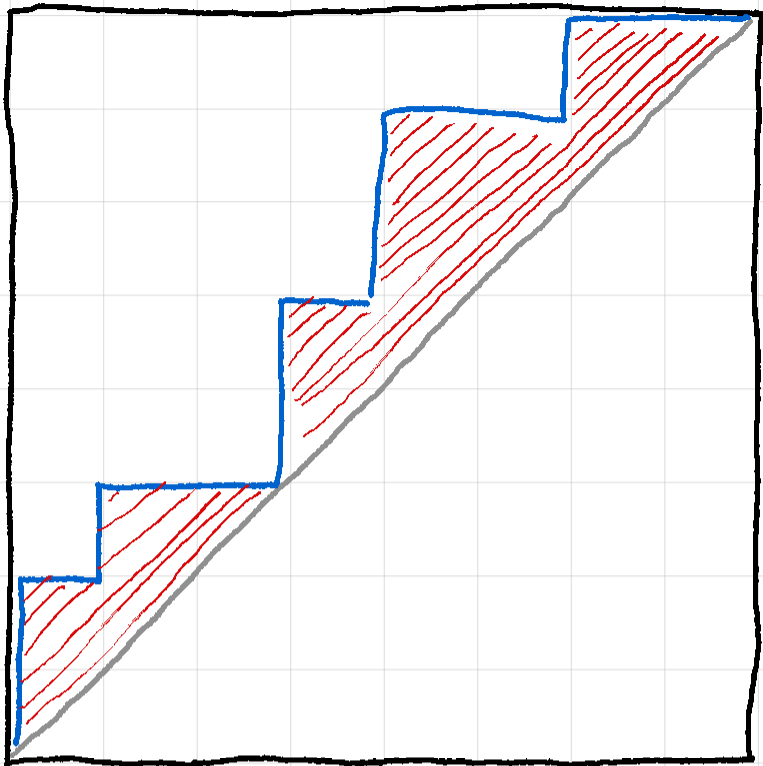
\includegraphics[width=0.8\textwidth]{graphics/area_under_dyck.png}
        \caption[][1.2cm]{En Dyck-stig med ytan under stigen streckad i rött.}
        \label{fig:area_under_dyck}
    \end{figure}

    Använd er kod för att, för varje $n$ mellan $1$ och $100$, skatta vad denna yta i genomsnitt blir, och rita upp en graf över hur den växer med $n$.
\end{xca}

\section{Genererande funktioner}

\begin{xca}
    Låt följden $d_{n,k}$ ges av att $d_{1,1} = d_{1,2} = 1$,
    $$d_{1,k} = d_{1,k-1} + d_{1,k-2} \quad \forall k \geq 3,$$
    samt
    $$d_{n,k} = \sum_{i=1}^k d_{n-1,i}$$
    för alla $n \geq 2$ och $k \geq 1$.

    Beräkna\sidenote[][-3cm]{Poängen med denna uppgift är så klart att den naiva metoden för att räkna ut detta skulle ta orimligt mycket tid, så man behöver använda någon smartare metod för att göra räkningen. För att hantera de rent algebraiska bitarna av räkningen med genererande funktioner kan nog ett lämpligt CAS vara behjälpligt, dessutom.

    Det finns antagligen mer än en möjlig metod, så här är två tips på möjliga riktningar: \emph{faltningar} och \emph{multivariata genererande funktioner}. (De senare har vi inte gått igenom i kursen, dock.)
    
    Den här övningen är definitivt svårare än den förra -- så en partiell lösning i vilken man t.ex. bara hittar en genererande funktion kan så klart ge partiella poäng.}
    $$d_{50000, 10^{10}} \mod 998244353.$$
\end{xca}

%\bibliography{references}
%\bibliographystyle{plainnat}

\end{document}
